%!TEX root = ../template.tex
%%%%%%%%%%%%%%%%%%%%%%%%%%%%%%%%%%%%%%%%%%%%%%%%%%%%%%%%%%%%%%%%%%%
%% chapter2.tex
%% NOVA thesis document file
%%
%% Chapter with introduction
%%%%%%%%%%%%%%%%%%%%%%%%%%%%%%%%%%%%%%%%%%%%%%%%%%%%%%%%%%%%%%%%%%%

\typeout{NT FILE chapter2.tex}%


\chapter{Atomic Structure Calculations}\label{cha:atom_calc}

In this chapter, the procedure that follows a standard atomic structure calculation will be discussed and explained in detail. Topics ranging from the usage of the \gls{MCDFGME} code to compute  quantities such as energy levels, orbital wavefunctions and transition rates, to the manner in which these parameters can be used in order to simulate a theoretical spectrum will be explored. All the information present in this chapter was obtained after a thorough study of \gls{MCDFGME}'s manual~\cite{Desclaux_Indelicato_2019}.


\section{The \gls{MCDFGME} code's capabilities}
As previously stated, \gls{MCDFGME} is a program that allows for not only solving the many-body problem for an atomic system while making the proper \gls{QED} energy corrections, but also for the computation of a great deal of atomic parameters. Consulting~\cite{mcdfWebsite}, one can see that these include, but are not limited to:

\begin{itemize}
    \item Energy level calculations.
    \item Multipole radiative transition probabilities.
    \item Auger transition probabilities.
    \item Photoionization cross-sections.
    \item Electronic impact excitation cross-sections.
    \item Orbital wavefunction overlaps between same and different atomic systems.
\end{itemize}
\todo{meter mais cenas}

% Quoting from the manual~\cite{Desclaux_Indelicato_2019}, these include:
% 
% \begin{itemize}
    % \item Total energy of a given state
    % \item Radiative and Auger transition probabilities
    % \item Photoionization cross-sections
    % \item Hyperfine structure constants
    % \item Landé factor
    % \item Electron impact excitation cross-sections
    % \item Stark effect
    % \item Parity non-conserving amplitude,
    % \item Magnetic part of the g 2 correction for antiprotons,
    % \item Scalar product of wave functions,
    % \item Shiff moment
    % \item Overlaps of orbitals between a n-electron and a n 1-electron state for Shake-off calculations
% \end{itemize}
%  


\section{The atomic system at study}

Before proceeding to the explanation behind every step of the calculations performed, a previous discussion on the reason behind them should be had.


The main purpose of this thesis is that of simulating a theoretical spectrum for Copper's x-ray emission lines when subjected to a near ionization threshold x-ray source.

At this energy range, two main processes will be responsible for an electron moving out of a core-shell: Resonant photoexcitation, and ionization.

While the simulation of the theoretical spectra for ionized Copper would be quite straightforward (due to the low shake probabilities at near ionization threshold energies, transitions for satellite states were not incorporated in the simulation), the more extensive calculation is that of resonant photoexcitation.

Aside from ionized Copper, multiple atomic structure calculations were performed for many of Copper's first excited state configurations in order to consistently account for all possible decays from excited states.

In total, and in addition to ionized Copper, 18 different standalone calculations were performed for the case in which the atomic system has undergone the process of an excitation of any one of the constituent electrons to one of the following orbitals:

\begin{itemize}
    \item 4s, 4p, 4d, 4f
    \item 5s, 5p, 5d, 5f, 5g
    \item 6s, 6p, 6d, 6f, 6g, 6h
    \item 7p, 8p, 9p
\end{itemize}


\subsection{Selecting all possible orbital configurations}

As to perform an atomic structure calculation, by making use of the \gls{MCDFGME} code, the system's electronic configuration is needed, hence why, for each calculation, all the possible one-hole and two-holes \footnote{These need to be considered due to describing the final state of the system after an Auger transition or Shake-off process. The Auger transition rates will be needed in order to compute the full width of the initial 1-hole level and diagram transitions.} configurations need to be provided, along with their respective labels which are used as identifiers of the orbital where the hole is present during the calculations. For example, in the case of ground state Copper that went through the process of the excitation of one of its electrons to the orbital 4p, there are many possibilities for the original orbital from where the electron came from. For this case, an example of all possible 1-hole and 2-holes configurations can be found in Annex~\ref{an:confs}. These are obtained by running a single hole, or two holes by all the orbitals present in the ground state configuration.


\section{Level Calculations}
Now that all configurations have been selected, the calculations can proceed.

The first and most influential, step needed in order to simulate theoretical spectra is the calculation of the level structure for all given configurations.

This, however, is no simple task. Besides the given configuration, an atomic level is described by two other quantum numbers.

\subsection{The level manifold}




Prior to proceeding with the discussion, it is important to establish some of the notation that will be used throughout this thesis. In this work, where hyperfine splitting is not accounted for, an atomic level will be described by three sets of quantum numbers. These will be the parameters that will influence the system's energy levels.

\paragraph{Hole orbital labels}


$\qty(n\ l_j)$ - This quantum number set is related to the system's electronic configuration and can be composed of one or more labels, indicators of the orbitals where electrons are missing. These labels may have no physical meaning on their own and are used in conjunction with files such as the one in Annex~\ref{an:confs} in order to retrieve the system's electronic configuration.
For demonstrative purposes, assuming an initial Copper's ground state configuration as a starting point, before any hole-generating processes, to be $1\text{s}^2\ 2\text{s}^2\ 2\text{p}^6\ 3\text{s}^2\ 3\text{p}^6\ 3\text{d}^{10}\ 4\text{s}^1$, the quantum number set in question can be used to describe various possible ionization configurations:

\begin{itemize}
    \item $1\text{s}^1\ 2\text{s}^2\ 2\text{p}^6\ 3\text{s}^2\ 3\text{p}^6\ 3\text{d}^{10}\ 4\text{s}^1  \rightarrow \qty(1\text{s})$
    \item $1\text{s}^1\ 2\text{s}^1\ 2\text{p}^6\ 3\text{s}^2\ 3\text{p}^6\ 3\text{d}^{10}\ 4\text{s}^1 \rightarrow \qty(1\text{s},2\text{s})$
\end{itemize}




\paragraph{Total angular momentum number}


$J$ - This number is the indicator of the total angular momentum of the atomic system, resulting from the couplings between the electrons'  orbital angular momenta and spin. A single configuration can result in many coupling possibilities and, in turn, different values for $J$.

As an example, let's take that of Copper that underwent the excitation process of an electron from the 2p orbital to 4p, with an electron configuration of $1\text{s}^2\ 2\text{s}^2\ 2\text{p}^5\ 3\text{s}^2\ 3\text{p}^6\ 3\text{d}^{10}\ 4\text{s}^1\  4\text{p}^1 $. One can now easily observe there are three open orbitals, each with an uncoupled electron. The different coupling possibilities between these three electrons will generate four different possible total angular momentum values: $J=\sfrac{1}{2},\ \sfrac{3}{2},\ \sfrac{5}{2},\ \sfrac{7}{2}$. In table \ref{tab:tot_ang_mom}, a coupling example will be given for each of them.


\begin{table}[h!]
    \centering
    \caption{Total angular momentum generated by different couplings}
    \label{tab:tot_ang_mom}
    \rowcolors{1}{}{GhostWhite}
    \begin{tabular}{cc|cc|cc|c}
        \toprule \multicolumn{2}{c|}{2p}&\multicolumn{2}{c|}{4s}&\multicolumn{2}{c|}{4p}&Total/$J$\\
        $m_l$ & $m_s$ & $m_l$&$m_s$&$m_l$&$m_s$&$m_l+m_s$\\\midrule
        $1$&$-\sfrac{1}{2}$&$0$&$-\sfrac{1}{2}$&$1$&$-\sfrac{1}{2}$&$\sfrac{1}{2}$\\
        $1$&$\sfrac{1}{2}$&$0$&$-\sfrac{1}{2}$&$1$&$-\sfrac{1}{2}$&$\sfrac{3}{2}$\\
        $1$&$\sfrac{1}{2}$&$0$&$\sfrac{1}{2}$&$1$&$-\sfrac{1}{2}$&$\sfrac{5}{2}$\\
        $1$&$\sfrac{1}{2}$&$0$&$\sfrac{1}{2}$&$1$&$\sfrac{1}{2}$&$\sfrac{7}{2}$\\\bottomrule
    \end{tabular}
\end{table}

\paragraph{Lagrange multiplier} $\epsilon$ - Indicator of the eigenvalue for the state on which the calculation will be performed on. The need for this quantum number arises from the fact that, even for the same configuration and the same total angular momentum, there are many possible arrangements that yield these quantum numbers. As an example, for the same configuration used previously, and assuming a total angular momentum $J=\sfrac{5}{2}$, there are three different possible couplings that generate that value of angular momentum, as can be seen in table \ref{tab:epsilon}.


\begin{table}[h!]
    \centering
    \caption{Same total angular momentum generated by different configurations}\label{tab:epsilon}
    \rowcolors{1}{}{GhostWhite}
    \begin{tabular}{cc| cc | cc}
        \toprule\multicolumn{6}{c}{$J=\sfrac{5}{2}$}\\\midrule
        \multicolumn{2}{c|}{2p}&\multicolumn{2}{c|}{4s}&\multicolumn{2}{c}{4p}\\
        $m_l$ & $m_s$ & $m_l$&$m_s$&$m_l$&$m_s$\\\midrule
        $1$&$-\sfrac{1}{2}$&$0$&$\sfrac{1}{2}$&$1$&$\sfrac{1}{2}$\\
        $1$&$\sfrac{1}{2}$&$0$&$-\sfrac{1}{2}$&$1$&$\sfrac{1}{2}$\\
        $1$&$\sfrac{1}{2}$&$0$&$\sfrac{1}{2}$&$1$&$-\sfrac{1}{2}$\\\bottomrule
    \end{tabular}
\end{table}

This splitting of quantum numbers for a given configuration gives origin to the level manifold (Figure~\ref{fig:manifold}), reason why, even for a simple calculation, hundreds to thousands of levels need to be calculated. It is also of note that, for a given Total angular momentum value, $J$, there are $2J+1$ states associated to it due to the angular momentum projection. In the presence of an external \gls{EMF}, the hyperfine level structure would be observed, due to Zeeman and Stark's effects. However, for the purpose of this thesis, no external field was considered, and calculations were only done for the maximum total angular momentum projection value, with a $2J+1$ degeneracy taken into account in the following calculations.

\begin{figure}[h!]
    \centering
    \begin{tikzpicture}
        \draw (0,0)node[anchor=south]{$1\text{s}^2\ 2\text{s}^2 2\text{p}^5\ 3\text{s}^2\ 3\text{p}^6\ 4\text{s}^1\ 4\text{p}^1\ $}--(0,-1);
        \draw (-6,-1) -- (6,-1);
        \draw (-6,-1) -- (-6,-2) node [anchor=north]{$J=\sfrac{1}{2}$};
        \draw (-2,-1) -- (-2,-2)node [anchor=north]{$J=\sfrac{3}{2}$};
        \draw (2,-1) -- (2,-2)node [anchor=north]{$J=\sfrac{5}{2}$};
        \draw (6,-1) -- (6,-2)node [anchor=north]{$J=\sfrac{7}{2}$};
        \draw (6,-2.5) -- (6,-3)node [anchor=north, text centered, align=center, text width=2cm]{
            $\sfrac{-7}{2},\ \sfrac{7}{2}$
            
            $\sfrac{-5}{2},\ \sfrac{5}{2}$

            $\sfrac{-3}{2},\ \sfrac{3}{2}$

            $\sfrac{-1}{2},\ \sfrac{1}{2}$
            };
        \node at (4.75,-4.15){$m_J =$};
        \draw (2,-2.5) -- (2,-3.25)node [anchor=north, text centered, align=center, text width=2cm]{
            $\sfrac{-5}{2},\ \sfrac{5}{2}$
            
            $\sfrac{-3}{2},\ \sfrac{3}{2}$

            $\sfrac{-1}{2},\ \sfrac{1}{2}$
            };
        \node at (0.75,-4.15){$m_J =$};
        \draw (-2,-2.5) -- (-2,-3.5)node [anchor=north, text centered, align=center, text width=2cm]{
            $\sfrac{-3}{2},\ \sfrac{3}{2}$
            
            $\sfrac{-1}{2},\ \sfrac{1}{2}$
            };
        \node at (-3.25,-4.15){$m_J =$};
        \draw (-6,-2.5) -- (-6,-3.75)node [anchor=north, text centered, align=center, text width=2cm]{
            $\sfrac{-1}{2},\ \sfrac{1}{2}$
            };
        \node at (-7.25,-4.15){$m_J =$};
        \node[white] at (7.25,-4){$m_J =$};

        \node at (-6,-7) {$6+7+3+1= 17$ levels};
        \node at (4,-7) {$6\times 2+7\times 4+3\times6+1\times 8=66$ states};
        \draw (6,-5) -- (6,-6)node[anchor=north]{$\epsilon_{\text{max}=1}$};
        \draw (2,-4.75) -- (2,-6)node[anchor=north]{$\epsilon_{\text{max}=3}$};
        \draw (-6,-4.3) -- (-6,-6)node[anchor=north]{$\epsilon_{\text{max}=6}$};
        \draw (-2,-4.6) -- (-2,-6)node[anchor=north]{$\epsilon_{\text{max}=7}$};
    \end{tikzpicture}
    \caption{Splitting of quantum numbers for a given configuration.}
    \label{fig:manifold}
\end{figure}

In conclusion, an atomic level can be defined by the set of these three quantum numbers. In the notation used throughout this thesis, a level will be identified by:

\begin{equation}
    i\equiv \qty[(n\ l_j)_i;\ J_i;\ \epsilon_i],
    \label{eq:level_notation}
\end{equation}

And the energy of the level:

\begin{equation}
    E_i\equiv E \qty[(n\ l_j)_i;\ J_i;\ \epsilon_i],
\end{equation}



\subsection{Level calculation with \gls{MCDFGME}}
\todo{Mention that the program works by the means of an input f05 file}
\todo{Breit can be used as self consistent or perturbative}
\todo{Talk about Lorentz and Coulomb gauges}

A typical level calculation begins with the formatting of the input \verb|.f05| file. This file contains the necessary information and instructions the program needs for the computation that follows when the executable \verb|mcdfgme2019.exe| is called.

The input file has a certain input structure in which certain calculation parameters are defined. A previously tailored template input file is used, where, by default, the full Breit interaction is considered, with the magnetic and retardation parts, as well as vacuum polarization  included in the self-consistent process. Retardation is also applied to Lorentz's and Coulomb's gauges.

The template is now formatted in order to perform the calculation for the desired level. The element's atomic number and the electron configuration are selected with the former having the same format as in Annex~\ref{an:confs}. The double of the value of the  total angular momentum is then indicated (as not to work with non-integer values) and so is the Lagrange multiplier/eigenvalue.

There are many other parameters to chose in order to have the \verb|.f05| ready for the computation. These parameters, however, are not always the same, since occasionally different methods will have to be employed in order to reach convergence. Before these methods are discussed, it is necessary to provide an explanation as to how to evaluate the numerical convergence of the calculation:

\subsection{Level calculation with \gls{MCDFGME} - Alternative}

For a given set of quantum numbers, a relativistic \gls{MCDF} was performed using the \gls{MCDFGME} script. The code executes an iterative self-consistent field calculation, accounting for both Coulomb and Breit's interactions, including the magnetic and retardation parts for the latter. For \gls{QED} corrections, the formation of local potentials due to vacuum polarization was included in the self-consistent part of the calculation, while corrections due to self-energy were treated as perturbation. Furthermore, electron correlation was also accounted for by composing the antisymmetric wavefunction as a linear combination of state wavefunctions with mixing coefficients.

For executing the calculation, a previously tailored \verb|.f05| input file is prepared. In it, a calculation with all the previously mentioned interactions is set up, with the option of changing the initial trial wavefunctions and the parameters of the self-consistent calculation cycles. Throughout the calculation these wavefunctions will go through a variational process, changing until the optimal solution is reached, as can be observed in Figure~\ref{fig:WFcomp}.

\begin{figure}[h!]
    \centering
    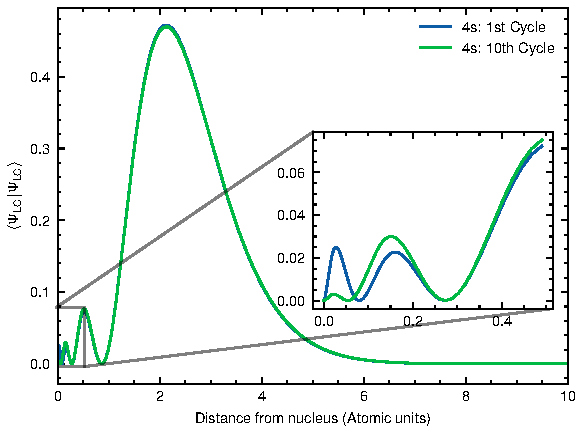
\includegraphics[width=.5\textwidth]{Chapters/Figures/Chapter2/WFcomp.pdf}
    \caption{ 4s Large component wavefunction after one and ten cycles of the self-consistent iterative process.}\label{fig:WFcomp}
\end{figure}\todo{Olha lá se não tens que fazer o quadrado disso}



\subsubsection{Evaluating the convergence}
After launching the \verb|mcdfgme2019.exe| executable, the computation will start, generating an output file with the \verb|.f06| extension, where the output will be written while the program is actively running.

One of the convergence benchmarks can already be evaluated while the calculation is being processed. Actively monitoring the output file with, as an example, the \verb|UNIX| command \verb|tail|, one can observe the output from the self-consistent cycles. Should the numerical method be diverging, warnings concerning sudden shifts in the wavefunction derivative may be displayed.

The calculation can also be aborted due to a numerical error. In this case, if the error occurred while running calculations for a certain orbital(s), this/these will be displayed in the output. 

The three other parameters used when evaluating if the convergence was successful can be checked only after the calculation is over:

\begin{itemize}
    \item Each cycle, a component of the level's energy is calculated through two different methods. These two values should be consulted for the last cycle and the absolute energy difference should be below a certain stipulated benchmark value ($1\ \si{\electronvolt}$).
    \item The wavefunction overlaps between each orbital sharing the same $l_j$ value are displayed, since these cases are the most probable of having a convergence error leading them not to be orthogonal. The convergence is considered acceptable if every value is lower than $10^{-6}$.
    \item For every orbital, the effective charge is calculated and displayed. This parameter is related to the shielding effect the charge of the electrons in other orbitals exert on the nuclear charge. If the calculation converged correctly, these values should never be equal to the extreme possible values: $1$ or $N$, where $N$ is the total number of electrons. For each orbital, this value should be close to an expected value \todo{Meter aqui ref de como calcular}.
\end{itemize}





\subsubsection{Level convergence methods}
\todo{Some text here. Mention the Optimize orbital method.}

\paragraph{First attempt at numerical convergence}
For the first calculation, by default, a simpler template file (Annex~\ref{an:first_cycle}) is used and a calculation of five self-consistent cycles is performed. All  trial orbital wavefunctions are initialized by wavefunctions calculated using the Thomas Fermi potential~\cite{thomas_1927}.





\paragraph{Second attempt at numerical convergence}
Should the first attempt have failed to reach convergence, a similar calculation is performed, keeping the previous parameters, but increasing the number of self-consistent cycles to 10, enforcing for each, an increasingly more precise accuracy and higher number of iterations. The template can be found in Annex~\ref{an:second_cycle}.


\paragraph{Third attempt at numerical convergence}
Should the previous two attempts have been made, and no convergence was reached, a new calculation needs to be made. In addition to the change cycle parameters, the parameters for some orbitals are to be altered. This can be done by altering the initial wavefunction to hydrogenics, or to a previously computed one. The method for solving the Dirac equation can also be changed for each chosen orbital. This final attempt can be quite time-consuming due to the many possibilities and combinations of methods to be employed for each orbital.


Since for every calculation thousands of levels need to be computed, a parallelized automation script was used. In total two scripts were used: a first one, previously written in \verb|bash| by one of the advisors, Jorge Machado, which used \verb|GNU|'s \verb|parallel|  command  for parallelization, was used for the first calculations performed; and for most of the calculations, a new script, developed in the scope of this thesis, written in \verb|Python| and employing an \verb|MPI| approach for the purpose of parallelization. This last one will be discussed further in the thesis.

In the total number of calculated 1-hole and 2-holes levels is displayed in Table~\ref{tab:tot_levels}.

\begin{table}[h!]
    \centering
    \caption{Total number of levels calculated. For all but the first row, the indicated orbital is the one where an electron was excited to.}
    \label{tab:tot_levels}
    \rowcolors{1}{}{GhostWhite}
    \begin{tabular}{c||c|c|c||c|c|c}
        \toprule Atomic&\multicolumn{3}{c||}{Number of levels}&\multicolumn{3}{c}{Number of hand-converged levels}\\
        System&1-hole&2-holes&Total&1-hole&2-holes&Total\\
        \midrule
        Cu$^{1+}$ & 19 &183&202&0&1&1\\ 
        4s& 10\\
        4p & 83 &1001 &1084&17&118&135\\
        4d & 107 &\\
        4f & 114\\
        5s & 33\\
        5p & 83\\
        5d & 107\\
        5f & 114\\
        5g & 115\\
        6s & 33\\
        6p & 83\\
        6d & 107\\
        6f & 114\\
        6g & 115\\
        6h\\
        7p & 83\\
        8p & 83\\
        9p & 83\\
        \midrule
        Total\\
        \bottomrule
    \end{tabular}
\end{table}
\missingfigure{Put level diagram example
}



\todo{Maybe put a plot of the calculated wavefunctions}
\section{Transition computations}

After all level computations have been performed, the next step towards the spectra simulation should be that of calculating level transitions. Any level that is not ground state will eventually decay into a more stable and less energetic one. This process is what eventually allows for the emission of x-ray radiation and Auger electrons.

When considering transitions between a given set of states, the transition energy and transition rate matrices are two 2D matrices of the greatest importance on spectra simulation, since their matrix elements contain the mentioned properties for all possible transitions across the set.

For an initial state denoted by $i$ and a final one by $f$ (using the notation from equation~\eqref{eq:level_notation}), the matrix elements are as follows:

For the energy matrix:

\begin{equation}
    E_{i,f} = E_i - E_f , 
\end{equation}

And now for the rate matrix:

\begin{equation}
    R_{i,f}=R\qty[(n,l_j)_i,J_i,\epsilon_i;(n,l_j)_f,J_f,\epsilon_f],
\end{equation}

\subsection{Diagram transitions}

Diagram transitions are associated with radiative transitions between two 1-hole states. For ionized systems, this kind of transitions are associated to the characteristic radiation from principal spectral lines such as $K_{\alpha},\ K_{\beta}, L$, etc. For this reason, they are the focal point of study for the work performed on this thesis.

Given a set of all $n_{1-\text{hole}}$ 1-hole levels, one must consider only transitions from higher to lower energetic states. Therefore, the total number of diagram transitions, not taking account level degeneracy, $N_{\text{diag}}$ can be simply calculated by the number of combinations of two 1-hole states:

\begin{equation}
    N_{\text{diag}} = \frac{n_{1-\text{hole}}!}{2\cdot\qty(n_{1-\text{hole}}-2)!},
\end{equation}



For the rate calculation, the same approach was taken as in the works of Guerra~\cite{Guerra2021} and Pinheiro~\cite{Pinheiro2023}, where the lack of orthogonality in the initial and final state due to numerical convergence is treated by the formalism present in Löwdin's work~\cite{Lowdin1955} and full orbital relaxation is allowed.

While \gls{MCDFGME} calculates transition rates for both Coulomb (length) and Lorentz (velocity) gauges\todo{needs to be checked}, only the length gauge calculated ones were used in this work. Rates are calculated for both Electric and Magnetic transitions and their many components (poles).

\subsection{Auger transitions}

As previous mentioned, these type of transitions are characterized by the transition's energy release coming in the form of an ejected electron, as opposed to x-ray radiation.

The set of initial and final states is now composed of the 1-hole and 2-hole sets. While for diagram transitions the total number of transitions could be calculated just by the number of elements in the set, in this case is not as simple, as the energy for every level has to be taken into account. The maximum number of possible transitions could be calculated by the product of the total number of 1-hole and 2-hole levels. The real number of transitions is, however, far away from this value.

Once again, the same procedure as in \cite{Guerra2021,Pinheiro2023} was followed. Given the energy of the transition, the free electron wavefunction is calculated for the same potential as the initial state. This time, no relaxation is included, as to only account for the ionization, and orthogonality between the free wave and the bound orbitals is enforced.


\subsection{Satellite transitions}
This type of transitions are related to radiative relaxation between two 2-hole states. They are, therefore processed the same as Diagram transitions.

While they might not be of great relevance for this thesis, some were still calculated as they can be useful for other works due to being equivalent to some diagram transitions for Copper following shake-up.


The total number of calculated transitions can be found in Table \ref{tab:tot_trans}:


\begin{table}[h!]
    \centering
    \caption{Total number of levels calculated. For all but the first row, the indicated orbital is the one where an electron was excited to.}
    \label{tab:tot_trans}
    \rowcolors{1}{}{GhostWhite}
    \begin{tabular}{c||c|c|c||c}
        \toprule Atomic&\multicolumn{4}{c}{Number of transitions}\\
        System&Diagram&Auger&Satellite&Total\\
        \midrule
        Cu$^{1+}$ & 171 &968&16653\\ 
        4s& 45 \\
        4p & 3403 &\\
        4d & 5671 &\\
        4f & 6441\\
        5s & 528\\
        5p & 3403\\
        5d & 5671\\
        5f & 6441\\
        5g & 6555\\
        6s & 528\\
        6p & 3403\\
        6d & 5671\\
        6f & 6441\\
        6g & 6555\\
        6h\\
        7p & 83\\
        8p & -\\
        9p & -\\
        \midrule
        Total\\
        \bottomrule
    \end{tabular}
\end{table}


\subsubsection{Rate and Energy Matrices as a calculation quality evaluation tool}

Due to \gls{MCDFGME} applying a numerical method, even after employing the optimize orbital for level calculation, the results obtained may not be accurate. This way a method for helping visualize the quality of a calculation is by plotting the rate matrix for the calculation.

The employment of this method was what lead to the decision not to perform the transition calculations for excitations to orbitals 8p and 9p, as well as excluding the results for excitation to 7p from the spectra simulation.

As an example, Figure~\ref{fig:4p_rm} represents the rate matrix for 4p-excited Copper:

\begin{figure}[h!]
    \centering
    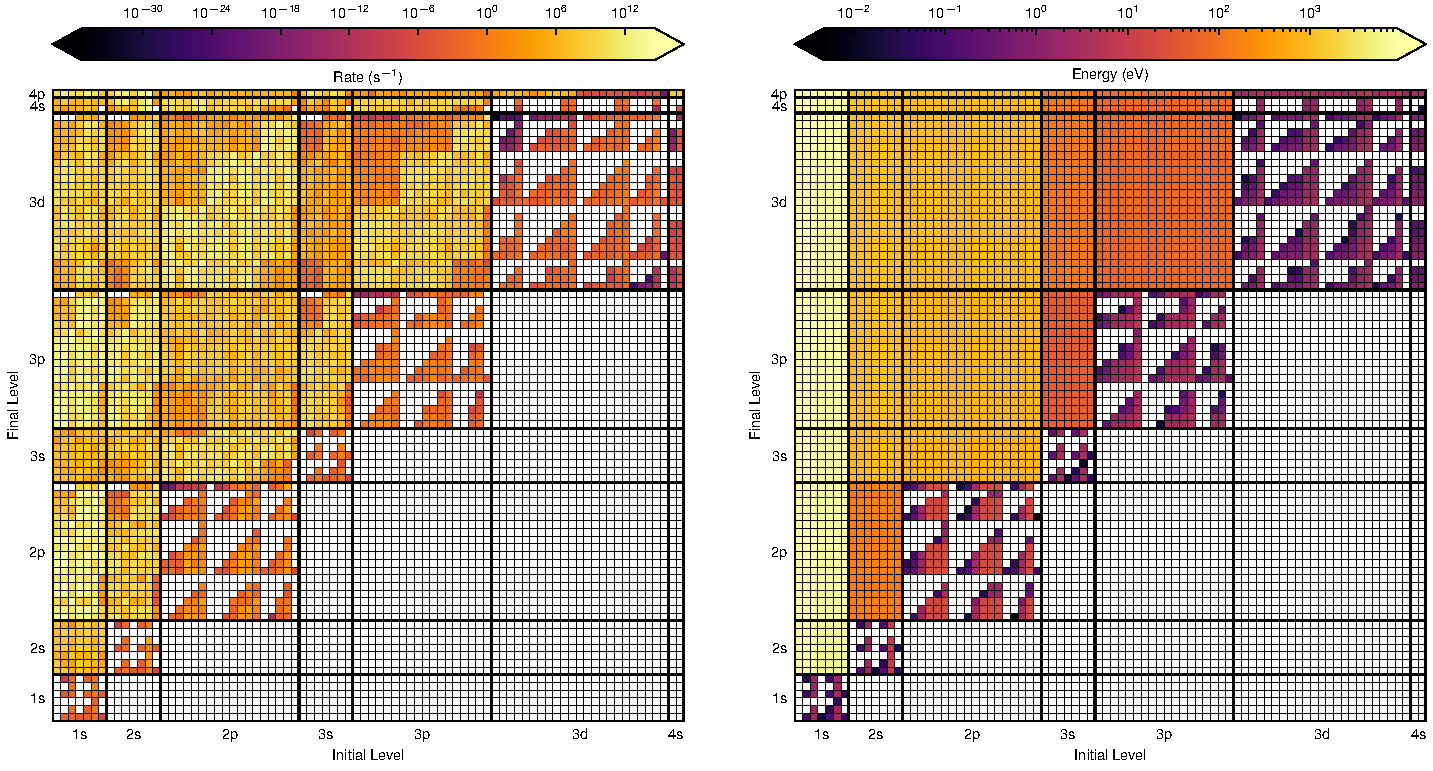
\includegraphics[width=\linewidth]{Chapters/Figures/Chapter2/4p_RM.pdf}
    \caption{Rate Matrix for 4p-excited Copper.}\label{fig:4p_rm}
\end{figure}

It is quite apparent that, as expected, only half the matrix elements are filled, due to transitions only occurring from higher to lower energy states. Moreover, transitions from np to 1s orbitals possessed the highest transition rate values, due to them composing the K spectrum, and the near-diagonal energy matrix elements present low energy values, due to being associated to similar state transitions. This city-like view is quite characteristic and can also be observed in all other successful calculations (consult Annex ??).

In the case of 7p-excited Copper, the fact that the obtained result is not correct is quite apparent just by looking at Figure~\ref{fig:7p_rm}:

\begin{figure}[h!]
    \centering
    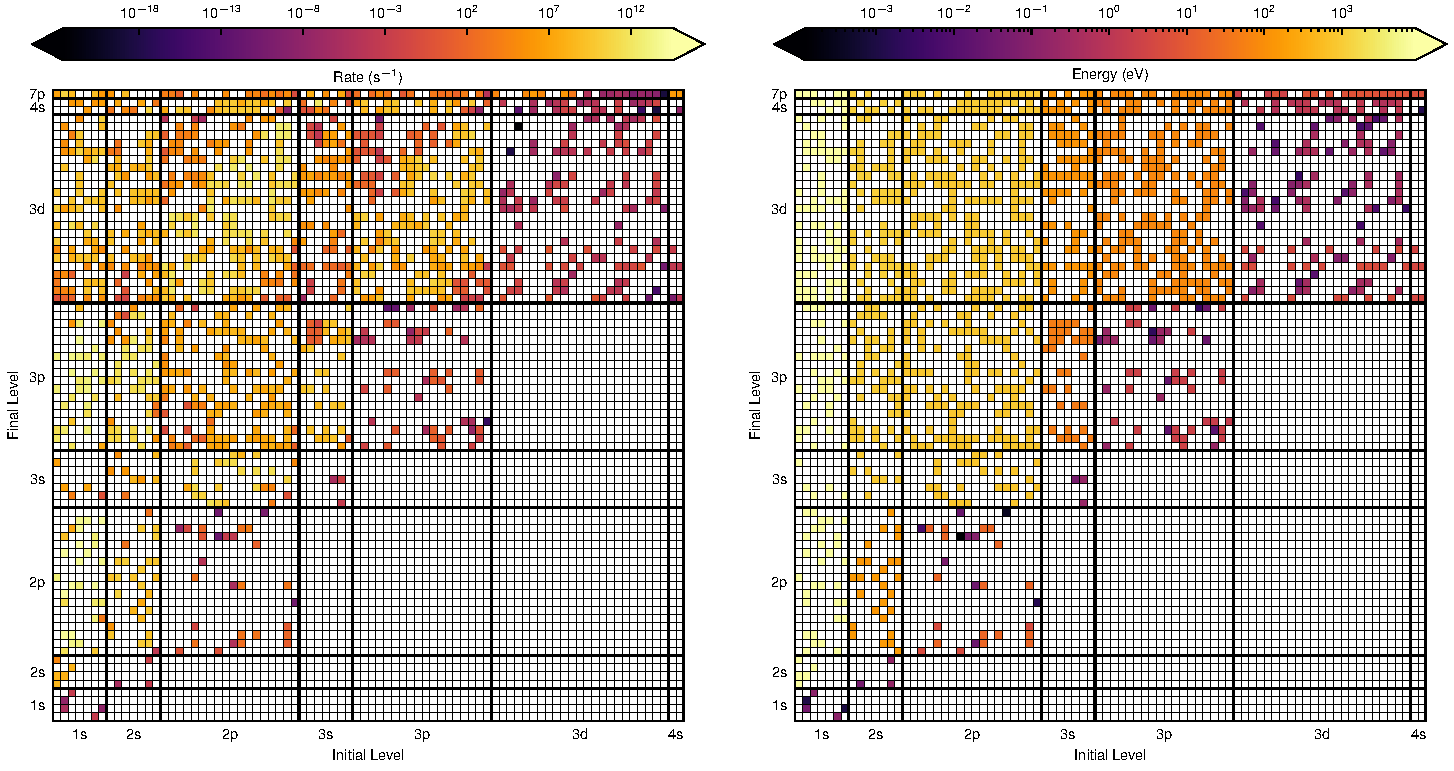
\includegraphics[width=\linewidth]{Chapters/Figures/Chapter2/7p_RM.pdf}
    \caption{Rate Matrix for 7p-excited Copper.}\label{fig:7p_rm}
\end{figure}

Here, the fact that the upper electron is in such a high orbital could have lead to an improper convergence during the level calculation. This may be responsible for the wrong level energies, which in turn influenced the calculated transitions. Due to this behavior, no more transition calculations were performed for excitations to upper orbitals.
\todo{ver o que raios se passou com o 7p}
